\documentclass[12pt]{article}
\usepackage[margin=1in]{geometry}
\usepackage{amsmath}
\usepackage{enumitem}
\usepackage{xcolor}
\usepackage{mathtools}
\usepackage{amssymb, amsthm}
\usepackage{tikz}
\usepackage{tkz-graph}
\usepackage{multicol}
\usetikzlibrary{arrows,automata}
\usepackage[nointegrals]{wasysym}

\newcommand{\red}[1]{\textcolor{red}{#1}}
\setlength\parindent{0pt}

\begin{document}
\title{MA-236: Homework 8}
\author{Rob Herley}
\maketitle

\begin{center}
I pledge my honor that I have abided by the Stevens Honor System.
\end{center}

Use the tree test to check if the following set of three sentences is consistent.  If yes, find an interpretation in which the sentences are all true.

$$Fa \quad \quad \forall x (\neg Fx \rightarrow Gx) \quad \quad \forall x Gx$$

\begin{center}
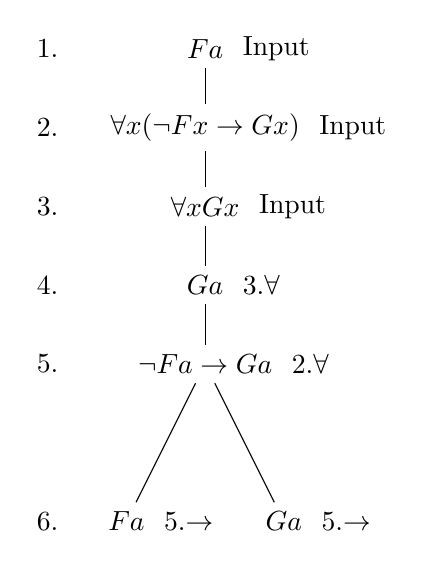
\begin{tikzpicture}
\draw (0,0)      node (11)                       {1.};
\draw (2cm,0)    node (13) [label=right:Input] {$Fa$};

\draw (0,-1cm)   node (21)                      {2.};
\draw (2cm,-1cm) node (23) [label=right:Input] {$\forall x (\neg Fx \rightarrow Gx)$};
\draw (13) -- (23);

\draw (0,-2cm)   node (31)                      {3.};
\draw (2cm,-2cm) node (33) [label=right:Input]{$\forall x Gx$};
\draw (23) -- (33);

\draw (0,-3cm)   node (41)                      {4.};
\draw (2cm,-3cm) node (43) [label=right:3.$\forall$]{$Ga$};
\draw (33) -- (43);

\draw (0,-4cm)   node (51)                      {5.};
\draw (2cm,-4cm) node (53) [label=right:2.$\forall$]{$\neg Fa \rightarrow Ga$};
\draw (43) -- (53);

\draw (0, -6cm) node (61)                       {6.};
\draw (1cm,-6cm) node (62) [label=right:5.$\to$]{$Fa$};
\draw (3cm,-6cm) node (63)  [label=right:5.$\to$]{$Ga$};
\draw (53)--(62);
\draw (53)--(63);

\end{tikzpicture}
\end{center}

\begin{center}
Since the tree is open, the sentences are \textbf{consistent}.
\end{center}
\underline{Interpretation}
\begin{multicols}{2}
  Domain: $\{ \ p_1 \ \}$ \\
  $a$ names $p_1$ \\ \\
  $Fa =$ true \\
  $Ga =$ true 

  \columnbreak
  
  $Fa$ $\Rightarrow$ true \\ \\
  $\forall x (\neg Fx \rightarrow Gx)$ $\Rightarrow$ $\neg Fa \rightarrow Ga$ $\Rightarrow$ true \\ \\
  $\forall x Gx$ $\Rightarrow$ $Ga$ $\Rightarrow$ true

\end{multicols}






\end{document}

